\documentclass[sigconf, nonacm]{acmart}
\usepackage{pdfpages}
\usepackage{amsmath}
\newcommand*\textfrac[2]{
  \frac{\text{#1}}{\text{#2}}
}
%% complete the rights form.
\setcopyright{none}

%% These commands are for a PROCEEDINGS abstract or paper.
\acmConference[Dundee Computing Honours Project '22]{Computing Honours Projects '22: The University of Dundee Computing Project Showcase: '22.}{2022}{Dundee, UK}


%%
%% end of the preamble, start of the body of the document source.
\begin{document}

%%
%% The "title" command has an optional parameter,
%% allowing the author to define a "short title" to be used in page headers.
\title{Code Quality Metrics - Mid-term}


\author{Christy McCarron}
\email{cswmccarron@dundee.ac.uk}
\affiliation{%
  \institution{University of Dundee}
  \city{Dundee}
  \state{Scotland}
  \country{UK}
}

%%
%% The abstract is a short summary of the work to be presented in the
%% article.

\begin{abstract}
Your abstract will go here.
\end{abstract}


%% A "teaser" image appears between the author and affiliation
%% information and the body of the document, and typically spans the
%% page.
\begin{teaserfigure}
  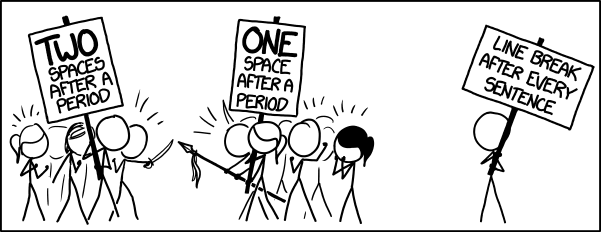
\includegraphics[width=\textwidth]{images/third_way.png}
  \caption{Third Way, xkcd}
  \Description{xkcd comic on language choices}
  \label{fig:thirdWay}
\end{teaserfigure}

%%
%% This command processes the author and affiliation and title
%% information and builds the first part of the formatted document.
\maketitle


% THIS IS THE MAIN PARTS OF THE DOCUMENT
\section{Introduction}
Code quality can be subjective, each person and organisation will have differing needs and wants when it comes to the quality of their code. But there are a many well defined areas that are as universal as can be.

test test
1234 aaa bbbb
\subsection{Secondary Part}
This is \textbf{another} part of my \textit{introduction}.

\begin{enumerate}
    \item This is the first item
    \item This is the second item
\end{enumerate}

This is another line of text that will go here

\begin{itemize}
  \item List entries start with the \verb|\item| command.
  \item Individual entries are indicated with a black dot, a so-called bullet.
  \item The text in the entries may be of any length.
\end{itemize}

\begin{table}[h]
\begin{tabular}{lll}
\hline
Colour & Score & Rating \\ \hline
Red    & 5     & B+     \\
Green  & 8     & A      \\ \hline
\end{tabular}
\end{table}
\section{Background}
In this project the student will focus on Static Analysis methods which are performed on source code this is as opposed to Dynamic Analysis which involves running the program and evaluating the quality while stepping through execution.

There are many ways to measure code quality but what we must establish is:
\begin{itemize}
    \item The code must do what it is meant to do.
    \item The code must be able to be tested.
    \item The code must be well documented.
    \item The code is readable and understandable.
    \item The code must be extendable.
\end{itemize}
\subsection{Tokenizing}
\begin{figure}[h]
    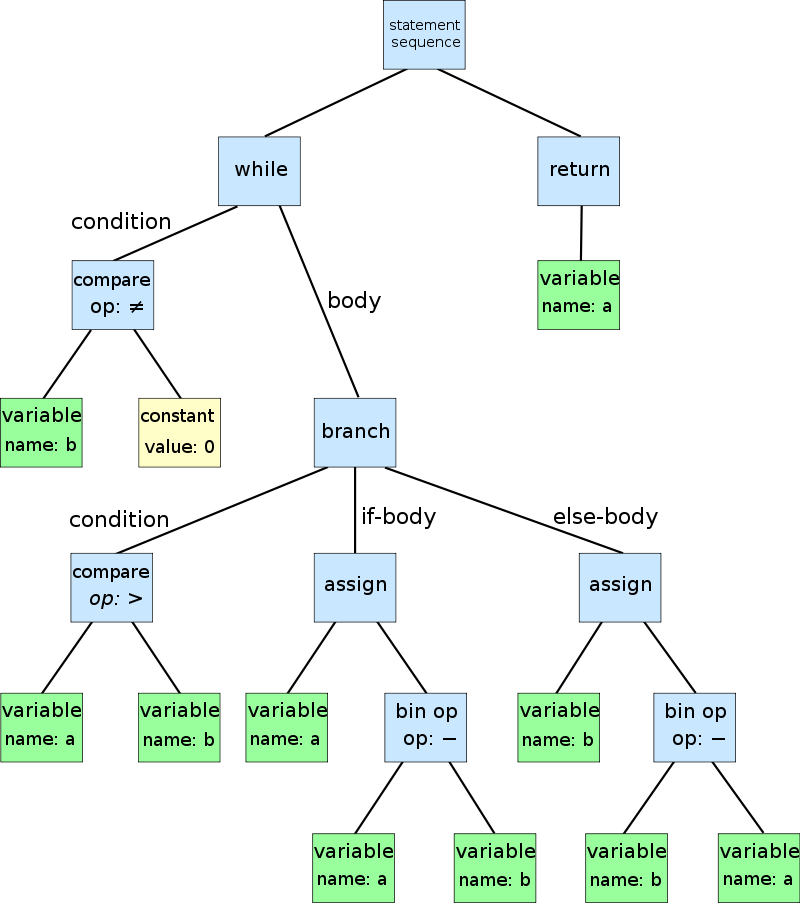
\includegraphics[width=.2\textwidth]{images/abstract-syntax-tree.png}
    \caption{Abstract Syntax Tree}
    \Description{graphical representation of abs of euclid algorithm}
    \label{fig:abs}
\end{figure}
In order to create a representation of the code we must tokenize the source code into it's component pieces and store this in an Abstract Syntax Tree. We can then use this representation of the code to preform our analysis.
The below code has been transformed into the AST in Figure.
\begin{verbatim}
    while b != 0
    if a > b
       a := a - b
    else
        b := b - a
    return a
\end{verbatim}
Each possibility in execution is converted to a tree which follows the path.
\subsection{Complexity Measures}
To measure code complexity there are a number of algorithms which measure different aspects of complexity of the code. These measure are agnostic to the language used so once the source code has been converted to an Abstract Syntax Tree any language may be evauluated by them.
\subsubsection{Halstead Complexity Measures}
In his 1977 book M.H. Halstead described a set of complexity measures. \cite{HalsteadComplexity}
\newline
These are described as such for any software program.
\begin{itemize}
    \item n\textsuperscript{1} : the number of unique operators
    \item n\textsuperscript{2} : the number of unique operands
    \item N\textsuperscript{1} : the total number of operators
    \item N\textsuperscript{2} : the total number of operands
\end{itemize}
Then several measures can be calculated from these.
\begin{itemize}
    \item Program Vocabulary    : n = n\textsuperscript{1} + n\textsuperscript{2}
    \item Program length        : N = N\textsuperscript{1} + N\textsuperscript{2}
    \item Calculated estimated program length : \^{N} = n\textsuperscript{1} log \textsubscript{2} n\textsuperscript{1} + n\textsuperscript{2} log \textsubscript{2} n\textsuperscript{2}
    \item Volume                : V = N * log \textsubscript{2} n
    \item Difficulty            : D =  $\textfrac{n\textsuperscript{1}}{2}$ * $\textfrac{N\textsuperscript{1}}{n\textsuperscript{1}}$
    \item Effort                : D * V
    \item Time required to program : T = $\textfrac{E}{18}$
    \item Number of delivered bugs : B = $\textfrac{V}{3000}$
\end{itemize}

\begin{verbatim}
    main()
    {
        int a, b, c, avg;
        scanf("%d %d %d", &a, &b, &c);
        avg = (a+b+c)/3;
        printf("avg = %d", avg);
    }
\end{verbatim}
In this example c program 
\begin{itemize}
    \item n\textsuperscript{1} : 12
    \item n\textsuperscript{2} : 7
    \item n : 19
    \item N\textsuperscript{1} : 27
    \item N\textsuperscript{2} : 15
    \item N : 42
    \item \^{N} : 12 log \textsubscript{2} 12 + 7 log \textsubscript{2} 7 = 62.67
    \item V : 42 * log \textsubscript{2} 19 = 178.4
    \item D : $\textfrac{12}{2}$ * $\textfrac{15}{7}$ = 12.85
    \item E : 12.85 * 178.4 = 2292.44
    \item T : $\textfrac{2292.44}{18}$ = 127.357 seconds
    \item B : $\textfrac{178.4}{3000}$ = 0.059
\end{itemize}

\subsubsection{Cyclomatic Complexity}
Cyclomatic Complexity(CC) is defined as 
\begin{verbatim}
    The number of linearly independant paths within a piece of code
\end{verbatim}
For example 
\newline
This piece of code has a CC of 1

\begin{verbatim}
    function test(a){
        return a
    }
\end{verbatim}
So does this
\begin{verbatim}
    function test(a){
        let b = a
        b = a*b
        b*=42
        return b
    }
\end{verbatim}
But when we add a control statement with 2 paths our control flow graph now contains 2 possible flows which gives us a CC of 2
\begin{verbatim}
    function test(a){
        if(a>2){
            return a
        }
        return b
    }
\end{verbatim}

This is an excellent measure to follow as not only does it make us segment our code for readability and extendability it ensures there are not too many test cases for a function.
\newline
McCabe suggested this in his 1976 paper \cite{cycloMaticComplexity}
\begin{verbatim}
    "Programmers have been required to calculate complexity as 
    they create software modules. When the complexity exceeded 
    10 they had to either recognize and modularize subfunctions 
    or redo the software. The intention was to keep the "size" 
    of the modules manageable and allow for testing all the 
    independent paths..."
\end{verbatim}
    
\section{Features}
The main features of the project are as follows
\begin{itemize}
    \item Web Interface with pseudo code editor
    \item Panel to control what analysis to perform
    \item Report Output
    \item Complexity analysis
    \item Syntactical analysis
    \item Code Smell Checking
    \item Readability checking
\end{itemize}

These items are also described in the User Stories Appendix



\section{Technology}
The student decided on using a node stack for the application, with a front end written in react fetching results from a node api.
\newline
This was chosen as it would allow for seemless use of commandline and web interface use of the program.
\section{Moving Forward}
\begin{figure}
    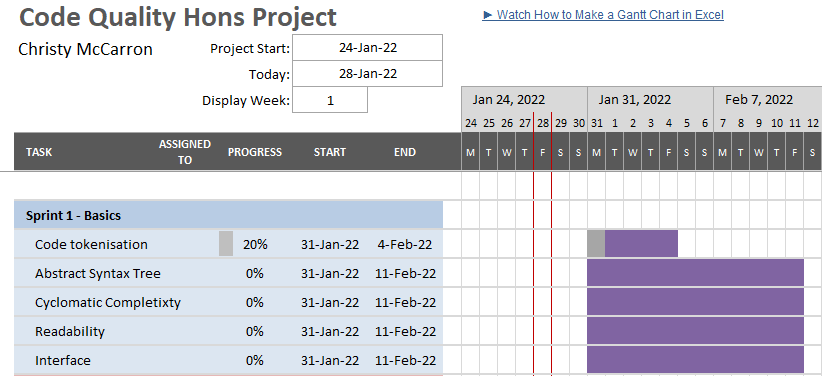
\includegraphics[width=.2\textwidth]{images/gantt.png}
    \caption{Gantt Sprint 1}
    \Description{gantt for sprint 1}
    \label{fig:gantt}
  \end{figure}
  Reflecting on the progress so far I believe that I have done a good amount of research which I will now apply to coding, I wish I had started prototying earlier as that would have made the planning much easier to estimate time.
  \newline
  As I am following agile I have made simple plans for sprint 1 where my sprints will be 2 weeks, after the end of sprint I will have a retrospective and review the progress completed in sprint 1.
  \newline
  I believe over the course of the project I should be able to complete every user story following this model.
  \newline
  The biggest pitfall that should be encountered is ensuring the abstract syntax tree is correct is this is the bed that everything else lies on, to ensure this it will be developed with a massive amount of unit and integration testing.




%%
%% The acknowledgments section is defined using the "acks" environment
%% (and NOT an unnumbered section). This ensures the proper
%% identification of the section in the article metadata, and the
%% consistent spelling of the heading.
% \begin{acks}
% To Robert, for the bagels and explaining CMYK and color spaces.
% \end{acks}

%%
%% The next two lines define the bibliography style to be used, and
%% the bibliography file.
\bibliographystyle{ACM-Reference-Format}
\bibliography{references}

%%
%% If your work has an appendix, this is the place to put it.
\appendix


\huge{\textbf{Appendices}}
\newline
\normalsize{Each appendix can be found either as a \underline{LINK} or in the sub folder with it's label, e.g. Appendix A is found in the path "/A/"}
\section{Control Flow Graph}
\section{Code Analyser Diagram}
\section{Compiler Diagram}
\section{User Personas}
\section{User Stories}
\section{Github Issues}
\url{https://github.com/aliveSurfin/code_quality/issues}
\section{MoSCoW Analysis}
\url{https://github.com/aliveSurfin/code_quality/projects/1}
\section{Value Risk}
\url{https://github.com/aliveSurfin/code_quality/projects/2}
\section{Combined MoscowValueRisk Priorities}
\url{https://github.com/aliveSurfin/code_quality/projects/3}
\section{T-Shirt Sizing}
\url{https://github.com/aliveSurfin/code_quality/projects/4}
\section{Source Code}
\url{https://github.com/aliveSurfin/code_quality/blob/main/development/code}
\section{Left Most Derivation Diagram}
\section{Right Most Derivation Diagram}
\section{Code Editor Initial Designs}
\section{Parser}
\url{https://github.com/aliveSurfin/code_quality/blob/main/development/code/parsing/parser/Parser.js}
\section{AST Types}
\url{https://github.com/aliveSurfin/code_quality/blob/main/development/code/parsing/parser/AST_CONST_TYPES.js}
\section{Tokeniser Folder}
\url{https://github.com/aliveSurfin/code_quality/tree/main/development/code/parsing/tokenizer}
\section{Parser Tests}
\url{https://github.com/aliveSurfin/code_quality/tree/main/development/code/parsing/parser/tests}
\section{Development Diary}
\url{https://github.com/aliveSurfin/code_quality/blob/main/development/diary/diary.md}
\section{Evaluation Features}
\url{https://github.com/aliveSurfin/code_quality/tree/main/development/code/parsing/evaluate}
\section{Final Product}
\url{https://code-quality-honours.herokuapp.com/}
\section{Code Coverage}
\section{Interview Notes}
\section{User Testing Results}


\end{document}
\endinput
%%
%% End of file `sample-sigconf.tex'.
